\section{Discussion and Conclusions}
In this paper,我们提出了DDPTransformer模型来解决sparse-view 下双域CT重建。并在实验部分证明它在LDCT-and-Projection-data数据集上的优异表现。但这并不能证明我们模型的鲁棒性。所以,我们从著名的"\emph{2016 NIH-AAPM-Mayo Clinic Low Dose CT Grand Challenge}"(2016aapm)\cite{mccollough2016tu}数据集中随机抽取了两位病人共1086个切片组成测试集进行测试。表5\ref{tab5}显示了对全部测试集进行测试的性能评价结果的均值和方差,可以看出在完全没有训练过的数据集上DDPTransformer的效果依然是最好的,和第二高的相比,PSNR在不同采样下分别高出了0.037dB(64view)和1.155dB(128view)。如图11\ref{fig11}所示,我们随机挑选了一个切片展示其视觉效果,并在图12中\ref{fig12}列出了他们的性能评价指标,通过对比我们发现DDPTransformer尽管RMSE值上并不是最好的,但在PSNR和SSIM上效果最好,并且在不同view下重建出的CT图整体质量更高。图13\ref{fig13}对于在放大的ROI下进行观察,DDPTransformer重建出CT图像在条纹伪影上处理的更好。因此,通过在2016AAPM数据集上的优异表现,我们验证了DDPTransformer的鲁棒性。\par
\begin{table}[H]
	\centering
	\resizebox{\textwidth}{!}{ 
	\begin{tabular}{cccc|ccc}
		\hline
		method & PSNR & SSIM & RMSE*100 & PSNR & SSIM &RMSE*100 \\ 
		\hline
		& \multicolumn{3}{c|}{64 views} & \multicolumn{3}{c}{128 views} \\ 
		\hline
		FBP & 29.9765$\pm$0.1209
		& 0.5416$\pm$0.0063
		& 0.1350$\pm$0.0035
		& 34.4040$\pm$0.0949
		& 0.7454$\pm$0.0061
		& 0.0446$\pm$0.0010 \\
		bilinear+FBP 
		& 30.4448$\pm$0.1365
		& 0.8206$\pm$0.0034
		& 0.0922$\pm$0.0029
		& 34.3314$\pm$0.1436
		& 0.9075$\pm$0.0021 
		& 0.0374$\pm$0.0012 \\
		FBPConvNet
		& 36.9814$\pm$0.1666
		& 0.8939$\pm$0.0032 
		& 0.0206$\pm$0.0008
		& 42.7887$\pm$0.0948
		& 0.9682$\pm$0.0004
		& 0.0054$\pm$0.0001 \\
		DD-Net 
		& 30.4719$\pm$0.0546
		& 0.8525$\pm$0.0015
		& 0.0900$\pm$0.0011
		& 33.7510$\pm$0.0444
		& 0.9039$\pm$0.0010
		& 0.0424$\pm$0.0004 \\			
		DP-ResNet 
		& 31.2974$\pm$0.1674
		& 0.8426$\pm$0.0036
		& 0.0746$\pm$0.0029
		& 35.3386$\pm$0.1026
		& 0.9120$\pm$0.0018
		& 0.0295$\pm$0.0007 \\
		Adaptive-Net 
		& 31.3441$\pm$0.2889
		& 0.8659$\pm$0.0041
		& 0.0738$\pm$0.0050
		& 35.3676$\pm$0.2762
		& 0.9284$\pm$0.0016
		& 0.0293$\pm$0.0018 \\
		EEDeepNet 
		& 32.4082$\pm$0.1377 
		& 0.8714$\pm$0.0024
		& 0.0578$\pm$0.0018
		& 43.9455$\pm$0.1820
		& 0.9750$\pm$0.0006
		& 0.0041$\pm$0.0002 \\
		DDPTransformer 
		& \textcolor{red}{37.0181}$\pm$0.3035
		& \textcolor{red}{0.9270}$\pm$0.0041
		& \textcolor{red}{0.0202}$\pm$0.0014
		& \textcolor{red}{45.1001}$\pm$0.3832
		& \textcolor{red}{0.9787}$\pm$0.0013
		& \textcolor{red}{0.0032}$\pm$0.0003 \\ 
		\hline
	\end{tabular}}
	\caption{2016AAPM数据集上不同方法的性能评价结果(均值$\pm$方差),最好的值用红色标出。}
	\label{tab5}
\end{table}
\begin{figure}
	\centering
	\includegraphics[height=4.67cm,width=18cm]{9.eps}
	\caption{2016AAPM数据集上的可视化结果,第一行为64views,第二行为128views}
	\label{fig11}
\end{figure}
\begin{figure}
	\centering
	\includegraphics[height=4cm,width=15cm]{16.eps}
	\caption{图11的性能评价指标。}
	\label{fig12}
\end{figure}
\begin{figure}
	\centering
	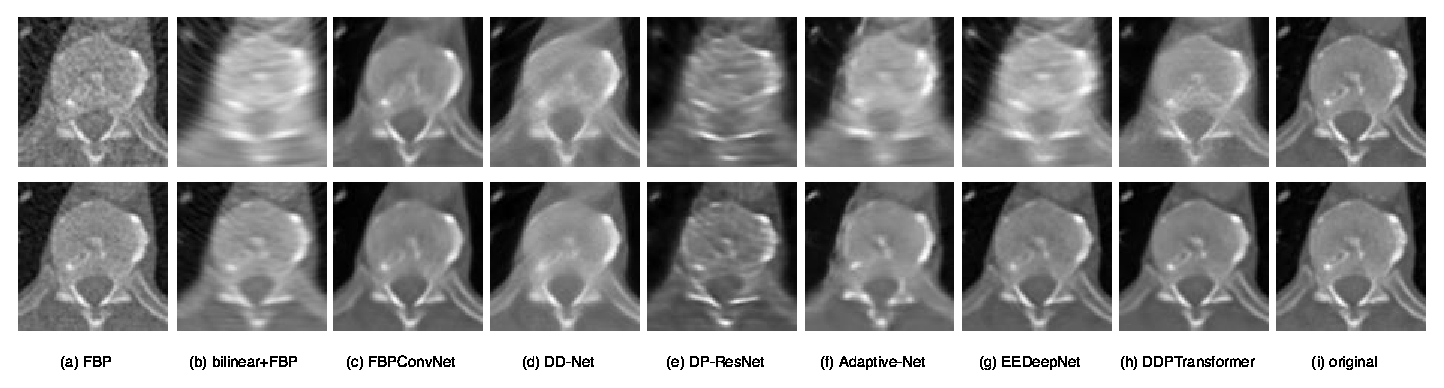
\includegraphics[height=4.67cm,width=18cm]{17.eps}
	\caption{图11(i)中红色框标记的缩放区域}
	\label{fig13}
\end{figure}







